\documentclass[8pt,a4paper]{article}
\usepackage{graphicx}
\usepackage{amsmath}
\usepackage{amsfonts}
\usepackage{amssymb,amsthm}
\usepackage{array}
\usepackage{setspace}
\spacing{0.75}
\usepackage[spanish, activeacute]{babel} %Definir idioma español
\usepackage[utf8]{inputenc} 
\usepackage{caption}
\usepackage{subcaption}

\voffset 0 cm \hoffset 0 cm \addtolength{\textwidth}{0cm}
\addtolength{\textheight}{0cm}\addtolength{\leftmargin}{0cm}

\begin{document}
%style file for ESANN manuscripts
\title{Procesamiento de texto manuscrito usando conjuntos de clasificadores}

%***********************************************************************
% AUTHORS INFORMATION AREA
%***********************************************************************
\author{
Emilio Samuel Aced Fuentes \\
Roberto Alcober Couso \\
Arturo Bl\'azquez P\'erez \\
Nicol\'as Trejo Moya \\
}
%***********************************************************************
% END OF AUTHORS INFORMATION AREA
%***********************************************************************

\maketitle

\section{Introducci\'on}
En este proyecto vamos a clasificar im\'agenes de letras manuscritas intentando predecir de forma correcta el s\'imbolo que representan.
Utilizaremos varios algoritmos de clasificaci\'on y los compararemos para encontrar los mejores resultados posibles, viendo diferencias de tiempos y  tasa de acierto.


\section{An\'alisis de los datos}
En el dataset provisto, est\'an representadas las 10 primeras letras del alfabeto(A-J), por tanto hay 10 clases posibles, las cuales hemos etiquetado en nuestra base de datos de 0 a 10 respectivamente.
Las imagenes nos vienen en un tamaño de $206\times150$ en escala de grises.


\begin{figure}[htbp]
	\centering
    \includegraphics[scale=0.5]{./sin_procesar/l00000_A.png}
    \caption{Ejemplo de una A}
\end{figure}



Como podemos observar las imagenes contienen ruido (manchas en el papel,rugosidades...), el cual podría dificultar la tarea de clasificación gravemente.Este problema lo hemos solucionado sometiendo a la imagen a diferentes tratamientos.

\subsection{Tratamientos}

Para todos los experimentos de este proyecto hemos umbralizado la imágen mediante otsu y posteriormente hemos realizado un filtro de mediana con un kernel cuadrado de tamaño 3.
Esto nos ha dado el siguiente resultado:
\begin{figure}[htbp]
	\centering
    \includegraphics[scale=0.5]{./procesado/l00000_A.png}
    \caption{Ejemplo de una A tratada}
\end{figure}

A continuación explicaremos los tratamientos que le hemos aplicado a las imágenes para reducir la complejidad del problema

\subsection{Atributos}
Teniendo en cuenta que las imágenes son matrices $206\times150$ tenemos un total de 30900 atributos, lo cual es una cantidad desorbitada, por ese motivo hemos decidido ver como afecta reducir la dimensión.
Las principales modificaciones que realizaremos a las imagenes para reducir su dimensionalidad son las siguientes:

\paragraph{Eliminar filas y columnas poco importantes}


Esto lo realizaremos mediante la selección de un umbral, con el cual consideraremos que las filas y columnas que tengan una cantidad menor de zona pintada que el umbral especificado no son de relevancia y por tanto las despreciaremos del problema

\begin{figure}[htbp]
    \centering
    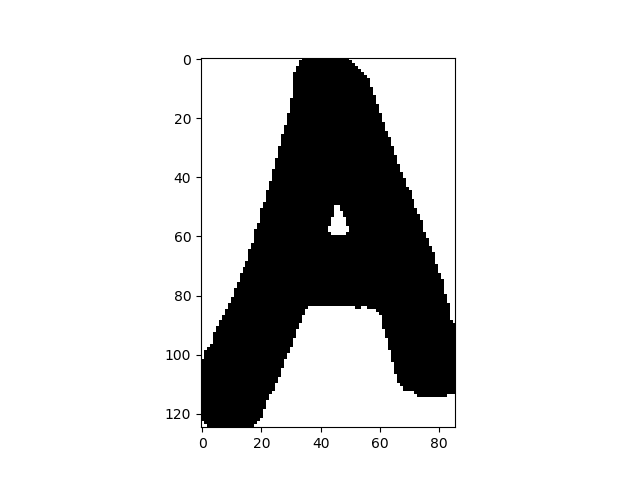
\includegraphics[scale=0.3]{./Arecortada.png}
    \caption{Ejemplo de una A recortada}
\end{figure}

\paragraph{Redimensionar la imágen interpolando}

Con el fin de evitar el aliasing (meter bordes que no existian al reducir una imágen) hemos redimensionado la imágen siempre aplicando un kernel gausiano previamente.

A continuacion mostraremos distintos valores de los tamaños de las imágenes que compararemos en nuestro estudio:

\begin{figure}[htbp]
   \centering
    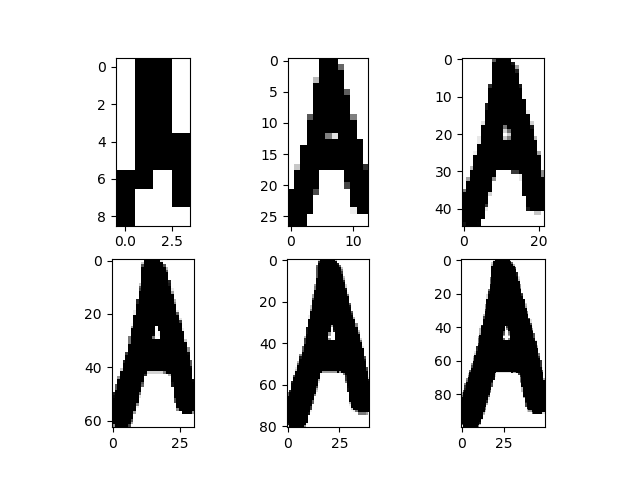
\includegraphics[scale=0.3]{./A_Variando_Tam.png}
    \caption{Varios tamaños de una A que usaremos}
\end{figure}


\section{Modelos}

Usaremos los siguientes clasificadores en este trabajo:
\begin{enumerate}
\item Random Forest
\item SVC
\item KNN
\end{enumerate}
en los cuales variaremos los tamaños de las imágenes y compararemos tiempos y tasa de aciertos para poder decidirnos por uno.

Para todos ellos destinaremos la mitad de los datos para train y la otra mitad para test.

\subsection{Random Forest}

Con random forest hemos encontrado que funciona muy bien incluso reduciendo mucho la dimension de los datos encontrando que la mejor tasa de acierto comparandola con el tiempo es reducir las imagenes a cuadrados $9\times4$ con 500 arboles de profundidad máxima 10 consiguiendo los siguientes resultados:
\begin{enumerate}
\item \textbf{Tasa de acierto}: 92.57$\%$
\item \textbf{Matriz de confusion}:

Como podemos ver en la matriz y la tabla Random Forest tiene como clases con menor precisión y sensibilidad B,I y J, sin embargo, hay una particularidad en los ejemplos donde hay una J, siempre que nos equivocamos al clasificar una J la predecimos como una I lo cual es razonable debido a la similitud de su grafía

\begin{figure}[htbp]
\centering
\begin{minipage}{.5\textwidth}
    \begin{tabular}{|c|c|c|} % <-- Alignments: 1st column left, 2nd middle and 3rd right, with vertical lines in between
    \hline
      \textbf{Clase} & \textbf{Precisión} & \textbf{Sensibilidad}\\
      \hline
      A & 0.93 & 0.99\\
      \hline
      B & 0.86 & 0.75\\
      \hline
      C & 0.97 & 0.99\\
      \hline
      D & 0.91 & 0.92\\
      \hline
      E & 0.95 & 0.92\\
      \hline
      F & 0.88 & 0.98\\
      \hline
      G & 0.96 & 0.97\\
      \hline
      H & 1    & 0.93\\
      \hline
      I & 0.88 & 0.87\\
      \hline
      J & 0.90 & 0.93\\
      \hline
    \end{tabular}
\end{minipage}%
\begin{minipage}{.5\textwidth}
\[
M=
  \begin{bmatrix}
    69 & 1 & 0 & 0 & 0 & 0 & 0 & 0 & 0 & 0 \\
    2 & 48 & 0 & 5 & 2 & 3 & 0 & 0 & 4 & 0 \\
    0 & 0 & 73 & 0 & 0 & 0 & 1 & 0 & 0 & 0 \\
    0 & 3 & 0 & 59 & 0 & 2 & 0 & 0 & 0 & 0 \\
    0 & 1 & 1 & 0 & 54 & 1 & 1 & 0 & 1 & 0 \\
    0 & 0 & 0 & 0 & 1 & 61 & 0 & 0 & 0 & 0 \\
    0 & 1 & 0 & 0 & 0 & 1 & 66 & 0 & 0 & 0 \\
    2 & 2 & 0 & 0 & 0 & 0 & 0 & 67 & 1 & 0 \\
    1 & 0 & 1 & 1 & 0 & 0 & 1 & 0 & 58 & 6 \\
    0 & 0 & 0 & 0 & 0 & 1 & 0 & 0 & 2 & 56 \\
  \end{bmatrix}
\]
\end{minipage}
\end{figure}

\item \textbf{Ejemplos de clasificacion}

\begin{figure}[h!]
\centering
    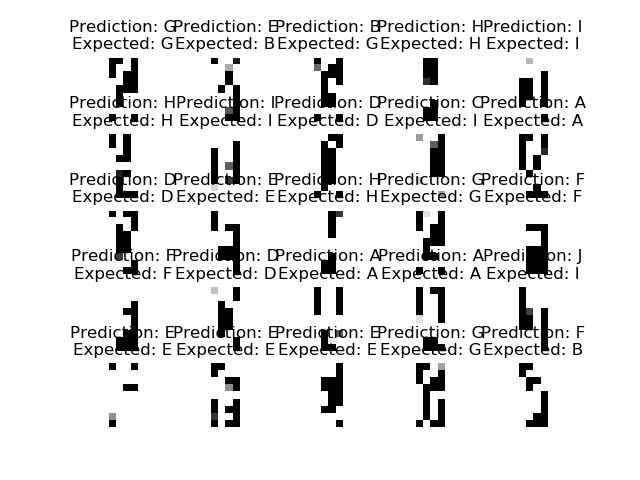
\includegraphics[scale=0.15]{./RandomForest_9_4.png}
    \caption{Ejemplos de clasificacion con random forest}
\end{figure}
\end{enumerate}

\subsection{Clasificador SVC}

Es el algoritmo que más tarda de los 3 con los que hemos experimentado, pero a su vez es el que consigue la mejor tasa de acierto. Para el ánalisis de resultados de este clasificador con estos datos decidimos reducir las imagenes a $100\times50$ con una gamma de 0.001 obteniendo los siguientes resultados:
\begin{enumerate}
\item \textbf{Tasa de acierto}: 96.21$\%$
\item \textbf{Matriz de confusion}:
Como se aprecia en la tabla y la matriz las letras en las que este clasificador tiene más problemas en reconocer son la J y la F dado que son las dos clases con menor precision. Por otro lado SVC que clasifica cinco Js y dos Es como Is y una A tres Ds y tres Fs como Bs, siendo B e I las clases con menor sensibilidad.
\begin{figure}[htbp]
\centering
\begin{minipage}{.5\textwidth}
    \begin{tabular}{|c|c|c|} % <-- Alignments: 1st column left, 2nd middle and 3rd right, with vertical lines in between
    \hline
      \textbf{Clase} & \textbf{Precisión} & \textbf{Sensibilidad}\\
      \hline
      A & 0.96 & 0.96\\
      \hline
      B & 0.95 & 0.89\\
      \hline
      C & 0.99 & 1\\
      \hline
      D & 0.94 & 0.97\\
      \hline
      E & 0.97 & 0.97\\
      \hline
      F & 0.93 & 1\\
      \hline
      G & 1    & 0.97\\
      \hline
      H & 1    & 0.97\\
      \hline
      I & 0.97 & 0.90\\
      \hline
      J & 0.92 & 0.97\\
      \hline
    \end{tabular}
\end{minipage}%
\begin{minipage}{.5\textwidth}
\[
  \begin{bmatrix}
    69 & 1 & 0 & 0 & 0 & 0 & 0 & 0 & 0 & 0 \\
    1 & 57 & 0 & 3 & 0 & 3 & 0 & 0 & 0 & 0 \\
    0 & 0 & 74 & 0 & 0 & 0 & 0 & 0 & 0 & 0 \\
    1 & 1 & 0 & 62 & 0 & 0 & 0 & 0 & 0 & 0 \\
    0 & 1 & 0 & 0 & 57 & 1 & 1 & 0 & 0 & 0 \\
    0 & 0 & 0 & 0 & 0 & 62 & 0 & 0 & 0 & 0 \\
    0 & 0 & 1 & 0 & 0 & 1 & 66 & 0 & 0 & 0 \\
    1 & 0 & 0 & 1 & 0 & 0 & 0 & 70 & 0 & 0 \\
    0 & 0 & 0 & 0 & 2 & 0 & 0 & 0 & 61 & 5 \\
    0 & 0 & 0 & 0 & 0 & 0 & 0 & 0 & 2 & 57 \\
  \end{bmatrix}
\]
\end{minipage}
\end{figure}

\item \textbf{Ejemplos de clasificacion}

\begin{figure}[htbp]
\centering
    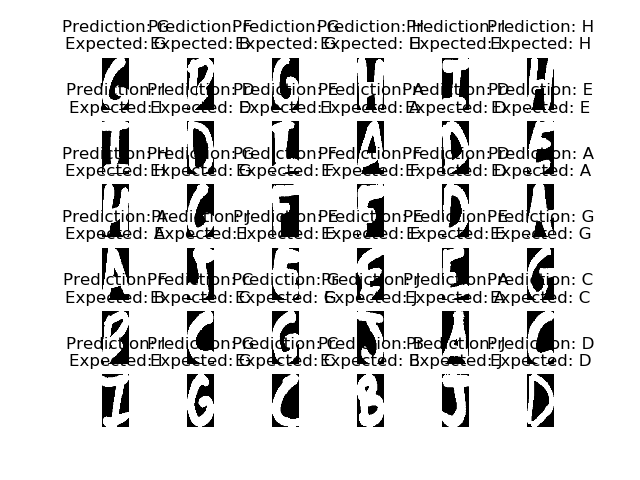
\includegraphics[scale=0.15]{./SVC100_50.png}
    \caption{Ejemplos de clasificacion con SVC}
\end{figure}
\end{enumerate}



\subsection{Clasificador KNN}

Como podremos ver más adelante este es un clasificador con el que conseguimos unos resultados medios, no tarda tanto como SVC ni tiene una tasa de acierto tan grande con imágenes tan reducidas como random forest pero aún así funcionó nos pareció suficientemente bueno como para incluirlo en la memoria
\begin{enumerate}
\item \textbf{Tasa de acierto}: 94.39$\%$
\newpage
\item \textbf{Matriz de confusion}:
	
Como podemos ver en la matriz, KNN se equivoca clasificando letras como B esto se puede apreciar en la segunda fila de la matriz de confusión donde vemos que ha clasificado una A, dos Ds , tres Fs y y 5 Is como B. Por ello se muestra una baja sensibilidad en la clase B. También es relevante mencionar que donde tiene más problemas a la hora de clasificar es en las letras C, F e I como se puede ver en sus correspondientes columnas y en que son las 3 clases con la menor precisión.
\begin{figure}[h!]
\centering
\begin{minipage}{.5\textwidth}
    \begin{tabular}{|c|c|c|} % <-- Alignments: 1st column left, 2nd middle and 3rd right, with vertical lines in between
    \hline
      \textbf{Clase} & \textbf{Precisión} & \textbf{Sensibilidad}\\
      \hline
      A & 0.97 & 0.99\\
      \hline
      B & 0.95 & 0.83\\
      \hline
      C & 0.91 & 1.00\\
      \hline
      D & 0.97 & 0.95\\
      \hline
      E & 0.98 & 0.88\\
      \hline
      F & 0.91 & 1.00\\
      \hline
      G & 0.98 & 0.91\\
      \hline
      H & 1    & 0.99\\
      \hline
      I & 0.85 & 0.91\\
      \hline
      J & 0.93 & 0.97\\
      \hline
    \end{tabular}
\end{minipage}%
\begin{minipage}{.5\textwidth}
\[
M=
  \begin{bmatrix}
    69 & 1 & 0 & 0 & 0 & 0 & 0 & 0 & 0 & 0 \\
    1 & 53 & 0 & 2 & 0 & 3 & 0 & 0 & 5 & 0 \\
    0 & 0 & 74 & 0 & 0 & 0 & 0 & 0 & 0 & 0 \\
    1 & 1 & 0 & 61 & 0 & 0 & 0 & 0 & 1 & 0 \\
    0 & 0 & 2 & 0 & 52 & 2 & 1 & 0 & 2 & 0 \\
    0 & 0 & 0 & 0 & 0 & 62 & 0 & 0 & 0 & 0 \\
    0 & 0 & 5 & 0 & 0 & 1 & 62 & 0 & 0 & 0 \\
    0 & 0 & 0 & 0 & 0 & 0 & 0 & 71 & 1 & 0 \\
    0 & 1 & 0 & 0 & 1 & 0 & 0 & 0 & 62 & 4 \\
    0 & 0 & 0 & 0 & 0 & 0 & 0 & 0 & 2 & 57 \\
  \end{bmatrix}
\]
\end{minipage}
\end{figure}



\item \textbf{Ejemplos de clasificacion}

\begin{figure}[htbp]
\centering
    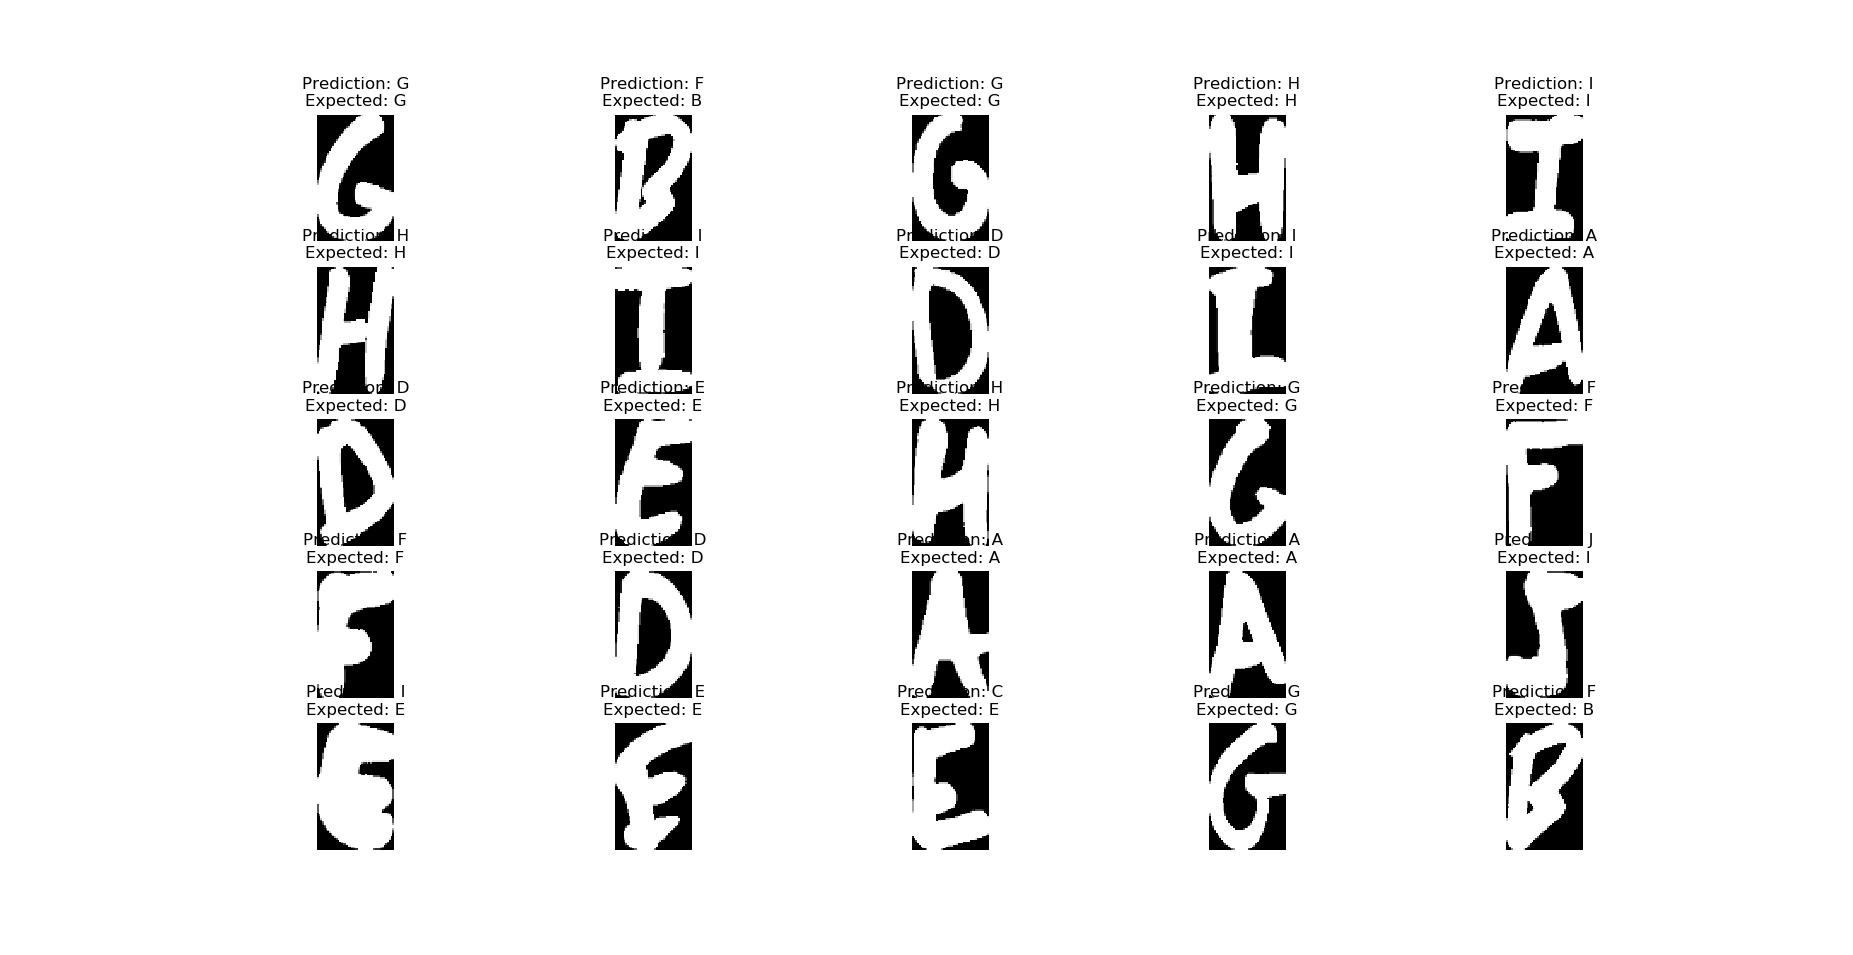
\includegraphics[scale=0.15]{./KNN_Ejemplos.png}
    \caption{Ejemplos de clasificacion con KNN}
\end{figure}
\end{enumerate}



\subsection{Comparar los clasificadores por su tasa de acierto}
Hemos decidido ir variando el número de parámetros que consideramos para ver como esto afecta tanto al tiempo de clasificacion como a la tasa de aciertos:

\begin{figure}[h]
\centering
\begin{minipage}{.5\textwidth}
  \centering
  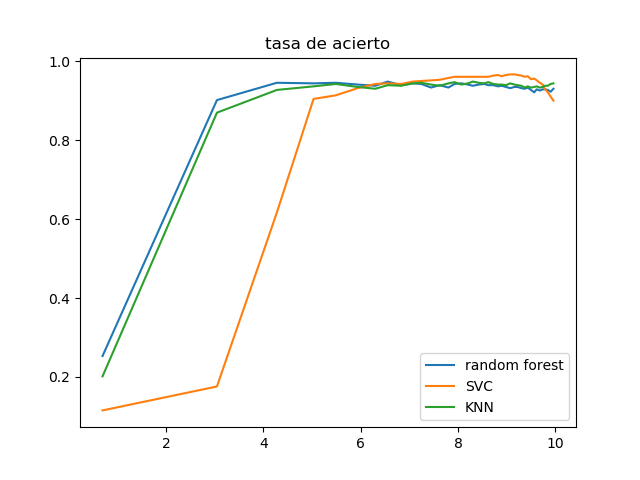
\includegraphics[width=0.8\linewidth]{./CompararAciertos.png}
  \captionof{figure}{Tasa de aciertos}
  \label{fig:test1}
\end{minipage}%
\begin{minipage}{.5\textwidth}
  \centering
  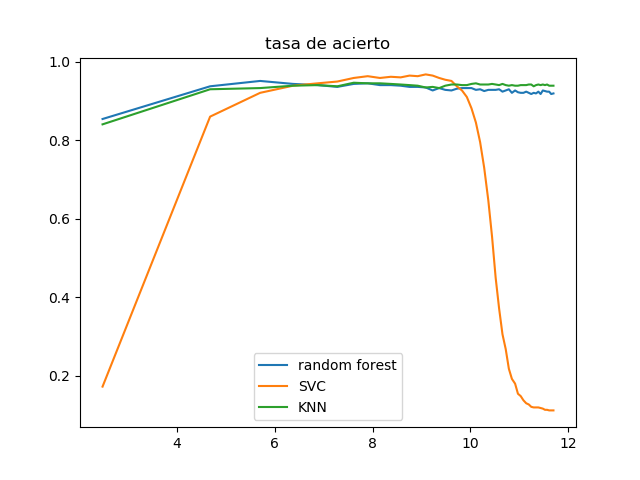
\includegraphics[width=0.8\linewidth]{./AciertosFinal.png}
  \captionof{figure}{Tasa de aciertos}
  \label{fig:test2}
\end{minipage}
\end{figure}

\newpage
En estas figuras muestra en el eje de las x la dimensión de los datos que usamos para clasificar en escala logaritmica en base e y en el eje y la tasa de acierto.
Como podemos ver a medida que aumentamos la cantidad de datos al usar SVC aumenta su tasa de acierto alcanzando un máximo con imágenes de tamaño $100\times50$, pero al contrario que con KNN y random forest, vemos que cuando empezamos a interpolar y a hacer las imágenes más grandes que el tamaño original su tasa baja.
Miremos la figura 11 donde hemos aumentando más aún el tamaño de las imágenes:
Como podemos ver su rendimiento baja notablemente, por eso concluimos en que SVC es menos robusto que KNN y Random Forest y por ello debemos tener cuidado a la hora de ver en qué set de datos lo usamos

\subsection{Comparar los clasificadores por su tiempo de ejecución}

En este apartado compararemos los tiempos de construir el clasificador y clasificar de KNN, SVC y Random Forest.



Como podemos ver en la figura 10 la diferencia entre los tiempos de ejecución en el limite son bastante notables encontrando que SVC es el más lento seguido de KNN y Random Forest el más rápido. El motivo por el cual SVC es el más lento es debido a su política de clasificación multiclase (one vs all) en la cual se ve obligado a aplicar el algoritmo 10 veces y escoger la clase que más se aproxime.

A continuación compararemos el tiempo que tardan con su tasa de acierto, con el objetivo de poder comparar para un limite de tiempo dado cual es mejor:



\begin{figure}[h]
\centering
\begin{minipage}{.5\textwidth}
  \centering
  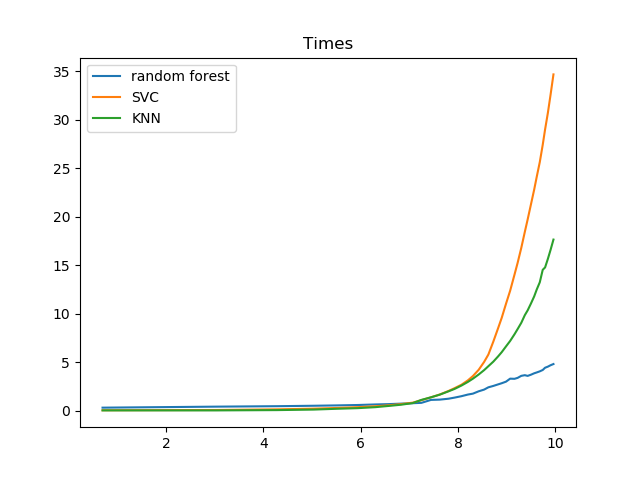
\includegraphics[width=1\linewidth]{./CompararTiempos.png}
  \captionof{figure}{Tiempos clasificación}
  \label{fig:test1}
\end{minipage}%
\begin{minipage}{.5\textwidth}
  \centering
  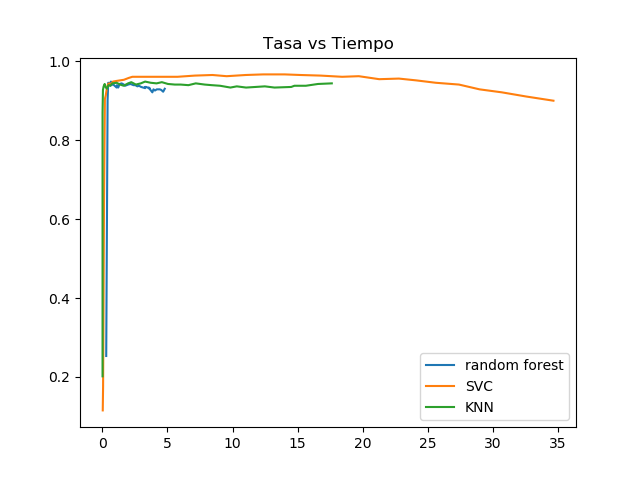
\includegraphics[width=1\linewidth]{./CompararAciertosvsTiempos.png}
  \captionof{figure}{Tasa acierto vs tiempos}
  \label{fig:test2}
\end{minipage}
\end{figure}


Finalmente compararemos solamente el tiempo de clasificación sin contar el tiempo de construir el clasificador.

\subsection{Conclusiones}
A la vista de los resultados obtenidos, dependiendo de nuestras necesidades, elegiremos distintos modelos. Si nuestra prioridad es la correcta clasificación de los datos y tenemos
una cantidad de tiempo ilimitada usaremos SVC pero, como hemos visto, es vulnearable cuando interpolamos la imagen para hacerla más grande por ello solo se debe aplicar en este problema an un numero de atributos entre 400 y 5000. Por otro, lado Random Forest es robusto a cambios en el espacio de atributos y alcanza una tasa de acierto bastante buena por ello es un buen candidato a la hora de resolver este problema. 

\subsection{Referencias}
Scikit-learn
\end{document}
